%%%% Paramétrage du TD %%%%
\def\xxnumchapitre{Chapitre 2 \vspace{.2cm}}
\def\xxchapitre{\hspace{.12cm} Révisions SLCI}

\def\xxcompetences{%
\textsl{%
\textbf{Savoirs et compétences :}\\
\vspace{-.4cm}
\begin{itemize}[label=\ding{112},font=\color{bleuxp}] 
\item .
%\item \textit{Mod3.C2 : } pôles dominants et réduction de l’ordre du modèle : principe, justification
\end{itemize}
}}

\def\xxfigures{
%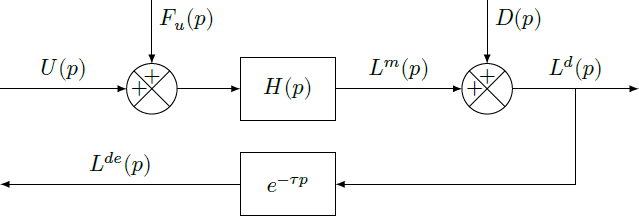
\includegraphics[width=.9\linewidth]{fig_02}
%\textit{}
}%figues de la page de garde

\def\xxtitreexo{Cisaille à découpe au vol}
\def\xxsourceexo{\hspace{.2cm} \footnotesize{D'après P. Dubois, C. Gamelon.}}

\def\xxactivite{{Colle 02} \ifprof  -- Corrigé \else \fi}


\input{\repRel/Style/pagegarde_TD}


\setlength{\columnseprule}{.1pt}

\pagestyle{fancy}
\thispagestyle{plain}

\vspace{4.5cm}

\def\columnseprulecolor{\color{bleuxp}}
\setlength{\columnseprule}{0.4pt} 
\setcounter{numques}{0}
%%%%%%%%%%%%%%%%%%%%%%%

\ifprof
\else
\begin{multicols}{2}
\fi


\section*{Mise en situation}
\ifprof
\else
\begin{obj}
\begin{itemize}
\item Identifier les paramètres du vérin.
\item Quantifier l'erreur de trainage et déterminer son impact sur le système.
\item Proposer des solutions pour la compenser.
\end{itemize}
\end{obj}
\begin{center}
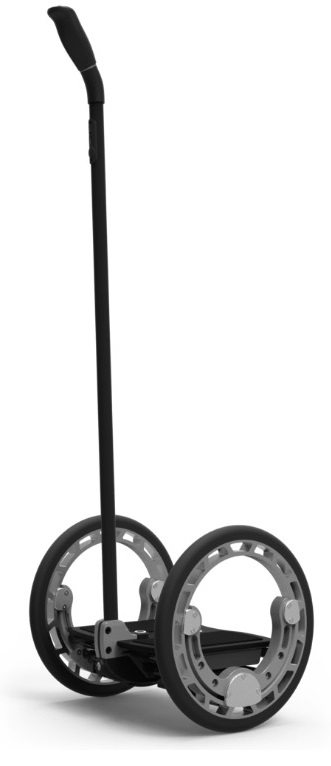
\includegraphics[width=\linewidth]{fig_01}
\end{center}

La machine, représentée par le schéma ci-dessus, permet de débiter en continu une bobine de tôle en tronçons de même longueur \footnote{
%\url{http://www.machinetool-video.fr/hot-rolled-steel-cut-to-lengh-line_2}
\url{https://goo.gl/azqSkT}}. La rotation continue à fréquence variable de la bobine impose à la tôle \textbf{(t)} une vitesse linéaire $v(t)$ par rapport au bâti \textbf{(b)} constante.
Les outils de découpe sont portés par la cisaille \textbf{(c)} qui est mise en mouvement par un vérin hydraulique.

En avançant, la tôle déplace le palpeur du capteur porté par la cisaille. Celui-ci délivre alors une tension $u(t)$ proportionnelle à l'écart de position entre la tôle et la cisaille. Un amplificateur transforme ce signal en courant d'intensité $i(t)$ pour commander un distributeur hydraulique qui fournit au vérin un débit d'huile $q(t)$. Au bout d'un certain temps, se déplaçant à la même vitesse, la cisaille et la tôle arrivent face à un détecteur qui déclenche la coupe. La tôle tombe, la cisaille recule jusqu'à son point de départ et attend que la tôle revienne en contact avec le palpeur pour recommencer un cycle. La position de la cisaille est ainsi « asservie » à la position de la tôle.

On notera par des majuscules les transformées de Laplace des fonctions du temps notées en minuscules.

Rappels : $\mathcal{L}\left[a\right]=\dfrac{a}{p}$, $\mathcal{L}\left[at\right]=\dfrac{a}{p^2}$ et $\mathcal{L}\left[e^{-at}\right]=\dfrac{1}{p+a}$. 

\fi
\section*{Schéma-bloc du système}
\ifprof
\else
On note : 
\begin{itemize}
\item $e(t)$ le déplacement de la tôle \textbf{(t)} par rapport au bâti \textbf{(b)};
\item $\varepsilon(t)$ le déplacement de la tôle par rapport à la cisaille \textbf{(c)};
\item $x(t)$ le déplacement de la cisaille par rapport au bâti. 
\end{itemize}
%Ces paramètres sont des fonctions du temps. 
On considère comme instant initial le moment où la tôle touche le palpeur. À cet instant $e$ et $x$ sont nuls. L'équation reliant les déplacements est donnée par :
$$\varepsilon(t)=e(t)-x(t).$$

%Question 1 : Ecrire la relation liant e, Ɛ et x.

Le capteur, l'amplificateur et le distributeur délivrent des signaux de sortie proportionnels à leurs signaux d'entrée. On notera $K_c$, $K_a$ et $K_d$ leurs gains respectifs. 
Soit  $H_v(p)=\dfrac{X(p)}{Q(p)}$ la fonction de transfert associée à l'ensemble vérin plus charge déplacée, ($X(p)$ est la transformée de Laplace du déplacement $x(t)$ et $Q(p)$ celle du débit $q(t)$).
\fi

\question{Représenter le schéma-blocs du système. Indiquer les grandeurs d'entrée et de sortie de chaque bloc.}

\ifprof \begin{corrige}
\begin{center}
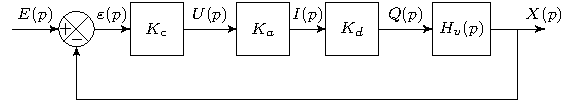
\includegraphics[width=.6\linewidth]{SchemaBlocs}
\end{center}
\end{corrige} \else \fi

\section*{Fonction de transfert de l'ensemble vérin et charge}
\subsection*{Équation de comportement dynamique}
\ifprof
\else
On note : 
\begin{itemize}
\item $m$ la masse totale mise en mouvement par le vérin;
\item $f$ le coefficient de frottement visqueux associé au déplacement de l'ensemble mobile. Les frottements créent un effort qui s'oppose au déplacement et qui est proportionnel à la vitesse : $F_f(t)=-f\dfrac{\text{d} x}{\text{d} t} \vect{x}$;
\item $\Delta p(t)$ la différence de pression entre les deux chambres $C_1$ et $C_2$ du vérin;
\item $S$ la surface du piston en contact avec l'huile.
\end{itemize}
En appliquant le principe fondamental de la dynamique à l'ensemble mobile en projection sur $\vect{x}$, on a : 
$$m\dfrac{\text{d}^2 x(t) }{\text{d}t^2}=S\Delta p(t)-f\dfrac{\text{d} x(t) }{\text{d}t}.$$
\fi

%\question{Appliquer le principe fondamental de la dynamique à l'ensemble mobile en projection sur $\vect{x}$.}

\subsection*{Fonction de transfert du vérin}
\ifprof
\else
Pour le type de vérin utilisé, le débit d'alimentation a pour expression : $q(t)=S\dfrac{\text{d}x(t)}{\text{d} t}+\dfrac{V}{2B}\dfrac{\text{d}\Delta p(t)}{\text{d}t}$. $V$ est le volume moyen d'une chambre et $B$ le module d'élasticité de l'huile, (ces deux paramètres sont des constantes).
\fi

\question{Transformer les deux équations précédentes dans le domaine de Laplace. En déduire l'expression de la fonction de transfert : $H_v(p)=\dfrac{X(p)}{Q(p)}$, que l'on mettra sous la forme : $H_v(p)=\dfrac{k}{p\left( ap^2 + bp + 1\right)}$}.
\ifprof \begin{corrige} ~\\
D'une part, $mp^2X(p)=S\Delta P(p)-fpX(p) \Leftrightarrow \dfrac{p\left(mp+f\right)}{S}X(p)=\Delta P(p) $.

D'autre part :
$Q(p)=SpX(p)+\dfrac{V}{2B}p\Delta P(p) \Leftrightarrow 2B\dfrac{Q(p)-SpX(p)}{Vp}=\Delta P(p) $.

On a donc : 
$\dfrac{p\left(mp+f\right)}{S}X(p) =
2B\dfrac{Q(p)-SpX(p)}{Vp}$
$\Longleftrightarrow
\dfrac{p\left(mp+f\right)}{S}X(p) +\dfrac{2BSpX(p)}{Vp}=
\dfrac{2BQ(p)}{Vp}$

$\Longleftrightarrow
\left(\dfrac{p\left(mp+f\right)}{S} +\dfrac{2BSp}{Vp}\right) \dfrac{Vp}{2B}=
\dfrac{Q(p)}{ X(p)}
\Longleftrightarrow
\left(\dfrac{p\left(mp+f\right)}{S} \dfrac{Vp}{2B}+Sp \right) =
\dfrac{Q(p)}{ X(p)}$.


On a donc, 
$H_v(p)
=\dfrac{1}{p\left(\dfrac{\left(mp+f\right)}{S} \dfrac{Vp}{2B}+S \right)}
=\dfrac{1}{p\left(\dfrac{Vm}{2BS}p^2+ \dfrac{fV}{2BS}p+S \right)}
=\dfrac{1/Q}{p\left(\dfrac{Vm}{2BS^2}p^2+ \dfrac{fV}{2BS^2}p+1 \right)}
$.

Au final, $k=\dfrac{1}{S}$, $a=\dfrac{Vm}{2BS^2}$ et $b=\dfrac{fV}{2BS^2}$.
\end{corrige} \else \fi

\subsection*{Détermination des paramètres canoniques à partir du diagramme de Bode}
\ifprof
\else
On pose $H_v(p)=\dfrac{K_v}{p\left( 1+\dfrac{2\xi}{\omega_0} p + \dfrac{p^2}{\omega_0^2} \right)}$. 

Une simulation numérique a permis de tracer le diagramme de Bode donné page suivante. On se propose de retrouver les valeurs de $K_v$, $\omega_0$ et $\xi$ à partir du diagramme.

\fi
%\begin{center}
%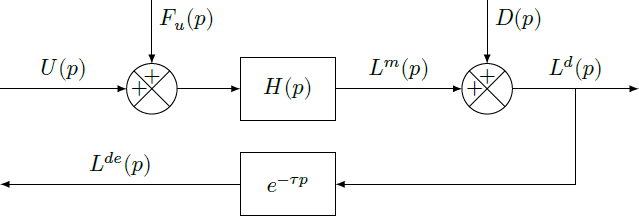
\includegraphics[width=\linewidth]{fig_02}
%\end{center}

\question{Donner l'expression littérale du gain fréquentiel en décibel $\text{GdB}(\omega)$ en fonction des notations $K_v$, $\omega_0$ et $\xi$, (ne pas développer le dénominateur pour le calcul du module de $H_v(j\omega)$). Quelle est sa valeur pour $\omega=\omega_0$ ?}

\ifprof \begin{corrige}
$H_v(j\omega )=\dfrac{K_v}{j\omega\left( 1+\dfrac{2\xi}{\omega_0} j\omega - \dfrac{\omega^2}{\omega_0^2} \right)}$

En conséquence,  $
G_{\text{dB}}\left(\omega \right)=20\log\left| \dfrac{K_v}{j\omega\left( 1+\dfrac{2\xi}{\omega_0} j\omega - \dfrac{\omega^2}{\omega_0^2} \right)} \right|
$
$
=20\log K_v- 20\log  \left| j\omega\right| - 20\log  \left| 1+\dfrac{2\xi}{\omega_0} j\omega - \dfrac{\omega^2}{\omega_0^2}  \right|
$

$
=20\log K_v- 20\log  \omega - 20\log  \left| \sqrt{\left(1- \dfrac{\omega^2}{\omega_0^2} \right)^2+\left( \dfrac{2\xi\omega }{\omega_0} \right)^2} \right|
$

Au final, 
$G_{\text{dB}}\left(\omega_0 \right)=
20\log K_v- 20\log  \omega_0 - 20\log 2\xi $.
\end{corrige} \else \fi

\question{Déterminer l'asymptote de la courbe de gain lorsque 
$\omega$ tend vers 0. Quelle est sa pente ?
Pour quelle valeur de $\omega$ coupe-t-elle l'horizontale à \SI{0}{dB} ?}

\ifprof \begin{corrige}
On a $G_{\text{dB}}\left(\omega \right)
=20\log K_v- 20\log  \omega - 20\log  \left| \sqrt{\left(1- \dfrac{\omega^2}{\omega_0^2} \right)^2+\left( \dfrac{2\xi\omega }{\omega_0} \right)^2} \right|$. 

Lorsque $\omega$ tend vers 0, le gain tend $20\log K_v- 20\log  \omega$.
 La pente est donc de \SI{-20}{dB/decade}. Elle coupe l'horizontale à \SI{0}{dB} en $\omega=K_v$.

\end{corrige} \else \fi

\question{Déterminer l'asymptote de la courbe de gain lorsque $\omega$ tend vers l'$\infty$. Quelle est sa pente ?	
Pour quelle valeur de $\omega$ coupe-t-elle l'asymptote précédente ?}


\ifprof \begin{corrige}
On a $G_{\text{dB}}\left(\omega \right)
=20\log K_v- 20\log  \omega - 20\log  \left| \sqrt{\left(1- \dfrac{\omega^2}{\omega_0^2} \right)^2+\left( \dfrac{2\xi\omega }{\omega_0} \right)^2} \right|$. 

Lorsque $\omega$ tend vers l'infini, le gain tend $20\log K_v- 20\log  \omega$, 
$G_{\text{dB}}$ tend vers 
$= 20\log K_v- 20\log  \omega - 20\log  \dfrac{\omega^2}{\omega_0^2} $
$= 20\log K_v- 20\log  \omega - 20\log  \omega^2 +20\log  \omega_0^2 $
$= 20\log K_v+ 40\log  \omega_0 - 60\log  \omega $.

La pente est donc de -60 dB/decade.

L'intersection des deux asymptotes a lieu quand 

$20\log K_v- 20\log  \omega= 20\log K_v+40\log  \omega_0 - 60\log  \omega$
$\Leftrightarrow \log  \omega= \log  \omega_0 $. Ainsi, l'intersection des asymptotes a lieu en $\omega=\omega_0$. 
\end{corrige} \else \fi

\question{Déduire des résultats précédents et du diagramme de Bode de $H_v(p)$ donné sur la feuille réponse les valeurs des paramètres $K_v$, $\omega_0$ et $\xi$ (on tracera les asymptotes avec leur pente réelle).}

\ifprof \begin{corrige}~\\

\begin{minipage}[c]{.45\linewidth}
\begin{center}
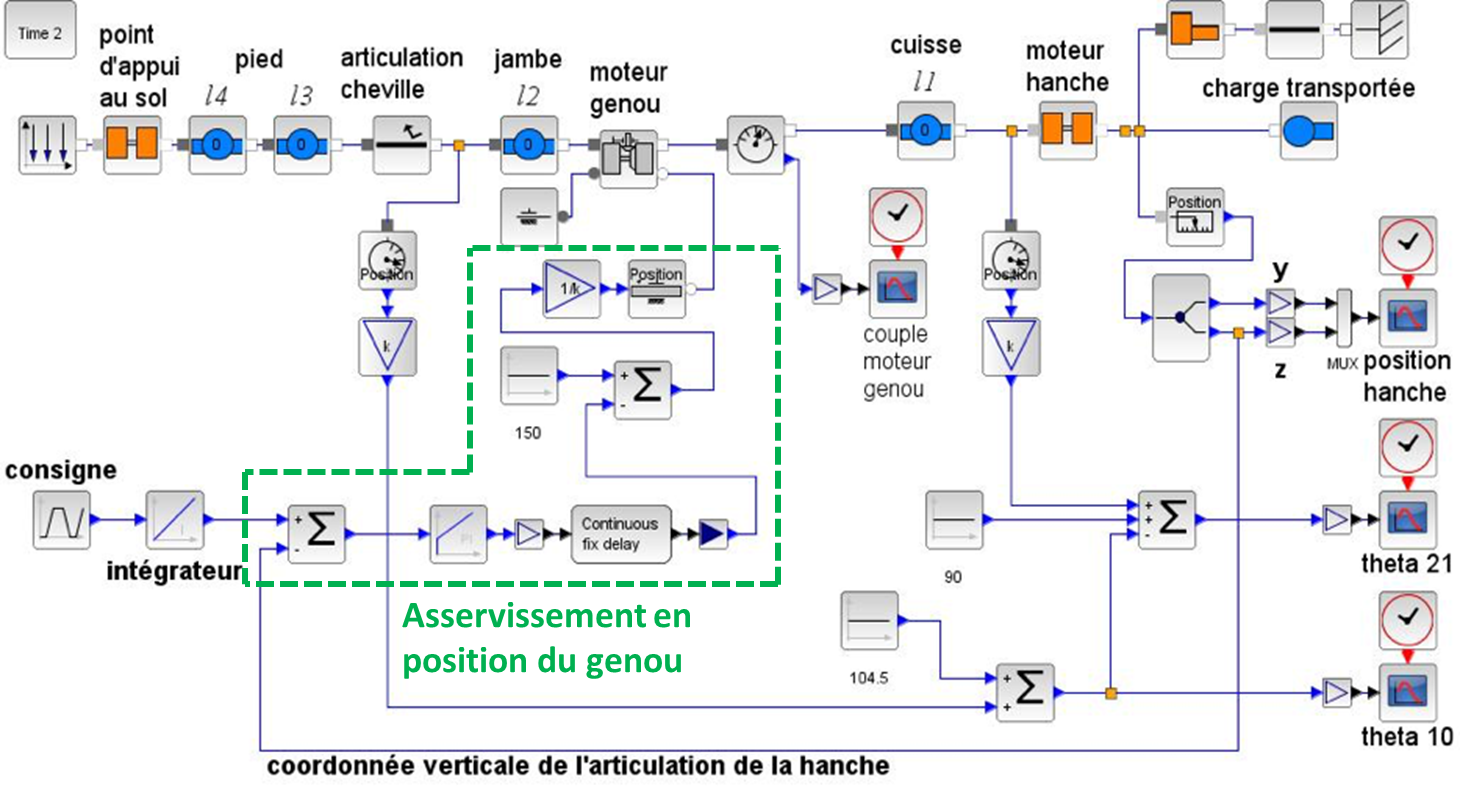
\includegraphics[width=.95\linewidth]{cor_01}
\end{center}
\end{minipage} \hfill
\begin{minipage}[c]{.45\linewidth}
Par lecture du graphe, on obtient $\omega_0=\SI{140}{rad/s}$ et $K_v=\SI{1000}{s.m^{-2}}$.

$G_{\text{dB}}\left(\omega_0 \right)=
20\log K_v- 20\log  \omega_0 - 20\log 2\xi 
\Leftrightarrow 37=20\log 1000 - 20\log  140 - 20\log 2\xi
\Leftrightarrow 37=60 - 20\log  140 - 20\log 2\xi
\Leftrightarrow \dfrac{37-60 + 20\log  140}{-20} =\log 2\xi
\Leftrightarrow  \xi \simeq 0,05
$.
\end{minipage}
\end{corrige} \else \fi


\question{Donner l'expression littérale de la phase $\varphi(\omega)$ en fonction des notations $\omega_0$ et $\xi$.	
Déterminer ses limites lorsque $\omega$ tend vers 0 et lorsque $\omega$ tend vers l'infini.	
Tracer le diagramme asymptotique de phase.	
Calculer les valeurs de la phase en degrés pour la pulsation propre $\omega_0$ puis pour \num{100} et \SI{200}{rad.s^{-1}}. Tracer la courbe de phase.}

\ifprof \begin{corrige} ~\\

$
\varphi\left(  \omega\right)
=\arg K_v- \arg \left( j\omega\right) - \arg  \left( 1+\dfrac{2\xi}{\omega_0} j\omega - \dfrac{\omega^2}{\omega_0^2}  \right)
=0-\dfrac{\pi}{2} - \arg  \left( \left( 1 - \dfrac{\omega^2}{\omega_0^2}\right) + \dfrac{2\xi\omega}{\omega_0} j \right)
$

Lorsque $\omega$ tend vers 0, $\varphi\left(\omega\right)$ 
tend vers $-\dfrac{\pi}{2}$. 

Lorsque $\omega$ tend vers l'infini,
$-\arg  \left( \left( 1 - \dfrac{\omega^2}{\omega_0^2}\right) + \dfrac{2\xi\omega}{\omega_0} j \right)$ tend vers $\pi$ donc $-\arg(...)$ tend vers $-\pi$.

\textit{Explication graphique de prof de SII...}
\begin{center}
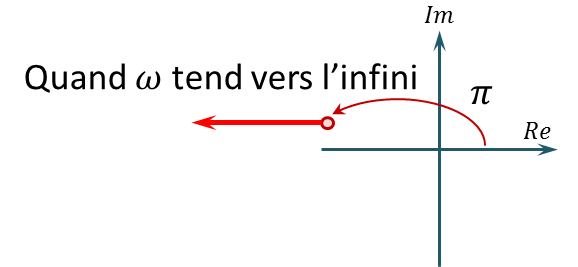
\includegraphics[width=.4\linewidth]{cor_02}
\end{center}
Au final, lorsque $\omega$ tend vers l'infini, $\varphi(\omega)$ tend vers $-\dfrac{3\pi}{2}$.

\end{corrige} 

\begin{center}
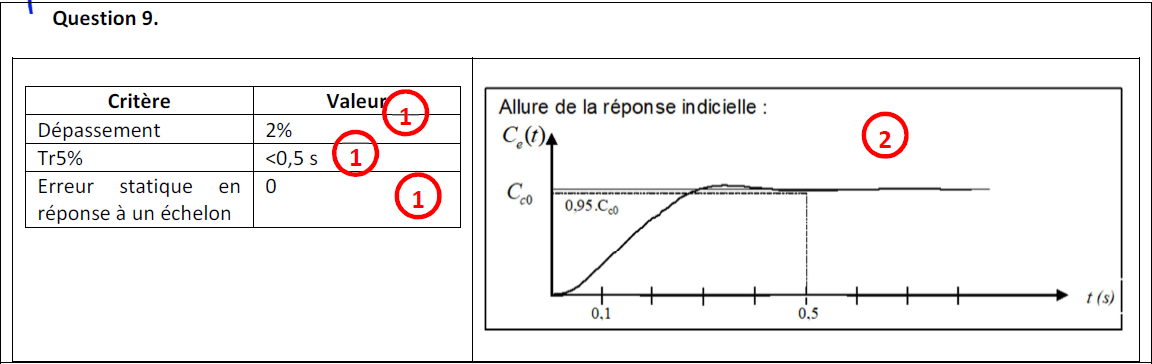
\includegraphics[width=.6\linewidth]{cor_03}
\end{center}

\else \fi




\subsection*{Détermination des gains $K_c$, $K_a$ et $K_d$}
\ifprof
\else
Pour que le système soit stable en boucle fermée on décide de régler le correcteur pour avoir une marge de gain de \SI{6}{dB}.
\fi

\question{Quelle valeur $K$ doit-on donner au produit des gains $K_c K_a K_d$ (préciser les unités).
On note $K_0$ le produit $KK_v$ (gain en boucle ouverte). Quelle est la valeur de $K_0$ ?
Quelle est la marge de phase ainsi obtenue ?}
\ifprof
\begin{corrige}
Étant donné l'exigence demandée, le gain de la FTBO doit être de \SI{-6}{dB} lorsque la phase vaut -180\degres.
On a déjà vu que pour cette phase, le gain décibel de $H_v$ vaut \SI{37}{dB}. Le gain dB vaut $20\log K + 20 \log |H_v|$. On cherche donc $K$ tel que $20\log K + 20 \log |H_v|=-6$. Au final, $K=\SI{7}{10^{-3}m^2.s^{-1}}$. Par suite, $K_0=\SI{7}{s^{-1}}$.
\end{corrige}
\else
\fi
\ifprof
\else
\begin{methode}
Cette question est un peu prématurée par rapport à notre avancée. Cependant, vous pouvez tentez d'appliquer la méthode suivante : 
\begin{enumerate}
\item Déterminer le gain (en dB) pour lequel la phase vaut -180\degres.
\item Chercher $K$ tel que $20\log|FTBO|=-6$.
\item Calculer $K_0$.
\end{enumerate}
\end{methode}
\fi

\subsection*{Erreur de traînage}
\ifprof
\else
On note :   $H(p)=\dfrac{X(p)}{\varepsilon(p)}$.
\fi

\question{Donner l'expression de l'écart $\varepsilon(p)$ en fonction de $E(p)$ et $H(p)$. La tôle se déplace à vitesse constante $v$, quelle est la transformée $E(p)$ de $e(t)$ ? Donner l'expression de $\varepsilon(p)$ en fonction de $v$ et des paramètres canoniques.}

\ifprof \begin{corrige}
On peut redémontrer le résultat suivant : $\varepsilon(p)=\dfrac{E(p)}{1+FTBO(p)}=\dfrac{E(p)}{1+H(p)}$.

Exprimons $\varepsilon(p)$ : $\varepsilon(p)=E(p)-X(p)=E(p)-H(p)\varepsilon(p)$; donc 
$\varepsilon(p)\left(1+H(p)\right)=E(p)\Longleftrightarrow \varepsilon(p)=\dfrac{E(p)}{1+H(p)}$.

Le consigne étant une vitesse, on a donc $E(p)=\dfrac{v}{p^2}$. On a donc : 
$\varepsilon(p)=\dfrac{v}{p^2}\dfrac{1}{1+\dfrac{K_vK_cK_aK_d}{p\left( 1+\dfrac{2\xi}{\omega_0} p + \dfrac{p^2}{\omega_0^2} \right)}}$.
\end{corrige} \else \fi

\question{On appelle erreur de traînage $\varepsilon_t$ la différence entre l'entrée et la sortie en régime permanent pour une entrée en rampe. Donner l'expression de $\varepsilon_t$. Faire l'application numérique avec $v = \SI{1}{m.s^{-1}}$ et $K_0 = 7$ (unité SI).}
\ifprof \begin{corrige}
L'entrée en vitesse précédente correspondant à une entrée en rampe, on a donc 
$
\varepsilon_t
= \lim\limits_{t\to +\infty} \varepsilon (t)
= \lim\limits_{p\to 0} p\varepsilon (p)
= \lim\limits_{p\to 0} p \dfrac{v}{p^2}\dfrac{1}{1+\dfrac{K_vK_cK_aK_d}{p\left( 1+\dfrac{2\xi}{\omega_0} p + \dfrac{p^2}{\omega_0^2} \right)}}
= \lim\limits_{p\to 0}  \dfrac{v}{p+\dfrac{K_vK_cK_aK_d}{\left( 1+\dfrac{2\xi}{\omega_0} p + \dfrac{p^2}{\omega_0^2} \right)}}
=\dfrac{v}{K_vK_cK_aK_d}
=\dfrac{1}{7}\simeq \SI{0,14}{m} $.
Pour compenser cette erreur, il suffit de régler la butée de la tôle à découper.
\end{corrige} \else \fi


\subsection*{Identification temporelle}
\ifprof
\else
On donne ci-dessous, le tracé de la courbe $x(t)$ obtenu à l'aide d'un logiciel de simulation.
Cette réponse est voisine de celle d'un premier ordre soumis à la même entrée.
Soit $F(p)=\dfrac{K_f}{1+Tp}$ la fonction de transfert du système du premier ordre associé.


\begin{center}
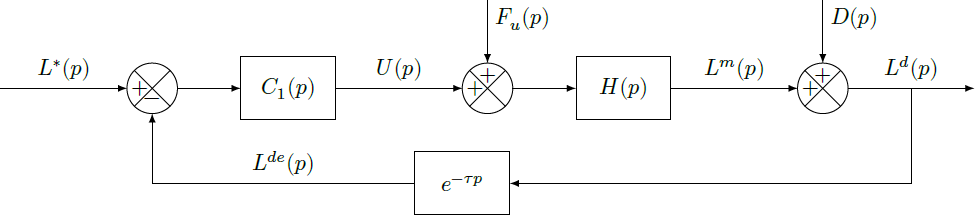
\includegraphics[width=\linewidth]{fig_03}
\end{center}
\fi

\question{Déterminer l'expression de la réponse temporelle de ce système soumis à une entrée identique à celle de la cisaille (déplacement de la tôle à vitesse constante : $v = \SI{1}{m.s^{-1}}$).}
\question{Déterminer les valeurs numériques de $K_f$ et $T$ à l'aide de relevés sur la courbe.}
\ifprof \begin{corrige}

Première solution : cf cours pour un système du premier ordre soumis à une rampe. 

Seconde solution : se raccrocher à ce que l'on sait (peut-être) pour un premier ordre soumis à un échelon... en effet, la rampe peut être assimilée à un premier ordre intégré. Ainsi, pour un système du premier ordre soumis à un échelon d'amplitude $v$, la valeur finale est $vK_f$. Ainsi, en intégrant, la pente en régime permanent sera de $vK_f$. 

La pente étant de 1 on a $K_f=1$. 

Reste à savoir que l'asymptote coupe l'axe des abscisses en $T$. Après lecture, $T=\SI{0,15}{s}$.
\end{corrige} 
\begin{center}
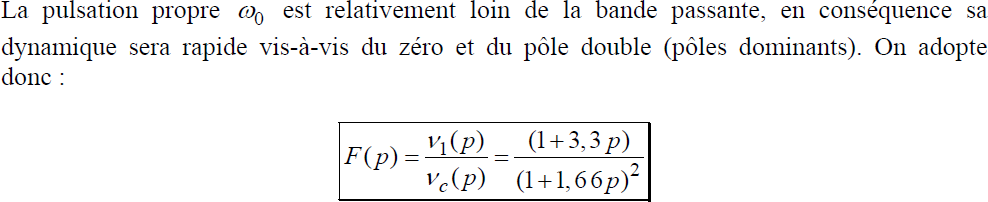
\includegraphics[width=.5\linewidth]{cor_04}
\end{center}
\else \fi





\question{Vérifier que l'on a la même erreur de traînage.}
\ifprof \begin{corrige}
Même erreur que précédemment.
\end{corrige} \else \fi

\question{Quel réglage peut-on envisager sur la cisaille pour compenser cette erreur ?}

\ifprof \begin{corrige}
Il est possible de décaler la butée de 14 cm et ainsi supprimer l'écart de trainage.
\end{corrige} \else \fi

\ifprof
\else
\end{multicols}
\fi
\ifprof
\else
\begin{center}
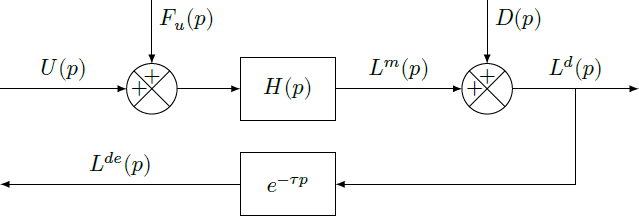
\includegraphics[width=\linewidth]{fig_02}
\end{center}
\fi
